\chapter {Planning}

\section {Chemical Ideas}


	\subsection{Rate of Reactions}

The definition of a rate of reaction is the rate at which reactants are converted into products. This has the mathematical equation of $Rate = \frac{\Delta Concentration}{Time}$. Finding the rate of reaction is obtained by studying the chemical kinetics of a specific reaction. The rate of reaction gives you important information such as, whether a reaction takes place at all, or how fast a reaction will occur. These chemical ideas are very important in the chemical industry as they allow for companies to reduce the cost and time in producing a product. The balanced chemical reaction only describes the stoichiometry between the reactants present and the amount of products that can be formed from them. Therefore rates are commonly used along side the balanced equation to get a further understanding of the reactions' process.

	\subsection{Factors that Affect the Rate of Reaction}

Increasing the concentration of the reactants increases the rate of reaction, up to a terminal concentration. This can be explained as two substances physically are unable to react with each other unless their particles come into contact with each other with enough kinetic energy (above the activation energy level). This means that if there is no contact between the particles, or the particles do not have enough kinetic energy, the rate of reaction will be zero. In contrast to this the higher the concentration of the reactants the more likely the particles are to collide above the activation energy per unit time allowing for a reaction to occur.

High temperatures allow for the particles within a system to have a greater kinetic energy. As the kinetic energy of the particles within a system increases, the particles move faster in the enclosed space, thus causing an increased chance of collision per unit time and also allowing for an increased chance of a collision above the activation energy. Virtually all reactions increase in rate if you increase the temperature. Decreasing the temperature has the opposite affect upon the rate of reaction (the rate decreases). In some systems, multiple reactions can take place, with each reaction happening at different temperatures. An example of this is the conversion of ethanol to diethyl ether, this occurs at around 100$^{\circ}$C, this is shown below:

$\mathrm{2CH_3CH_2OH}\xrightarrow{\mathrm{H_2SO_4}}\mathrm{CH_3CH_2OCH_2CH_3}+\mathrm{H_2O}$

However at 100$^{\circ}$C a different product is produced, ethylene$^1$.

$\mathrm{CH_3CH_2OH}\xrightarrow{\mathrm{H_2SO_4}}\mathrm{C_2H_4}+\mathrm{H_2O}$

Pressure only affects the rate of reaction if the reaction involves gases. Changing the pressure when a reaction involves only solids or liquids will have no effect on the rate of the reaction. Increasing the pressure of a gas is the same as increasing the gases concentration. If a given volume of gas is squeezed into a smaller volume the concentration is higher as shown by the equation:

 $p= \frac{n}{V}\times{RT}$

Where:
\begin{itemize}
\item p is pressure.
\item V is volume.
\item n is the number of moles.
\item R is the gas constant.
\item T is the temperature in K
\end{itemize}

Therefore this equation shows that as long as the temperature is constant, the pressure is directly proportional to the concentration. If you double one, you will also double the other$^2$.

Radiation is a form of energy and therefore it may speed up the rate of reaction as it provides the particles of the reactants with more energy, therefore allowing for more collisions above the activation energy per unit time. As the intensity of radiation increases, the particles absorb more energy and in turn the rate of reaction increases.

Surface area is important in chemical kinetics as increasing the surface area of a reactant will generally increase the rate of reaction. An example of this is iron, in solid form iron is stable enough to be used as solid blocks in building structures; however, in powder form a pyrotechnic composition can be created to form thermite, which when ignited by heat undergoes a vigorous exothermic reduction-oxidation reaction$^3$. The reason the rate of reaction increases as the surface area of reactants increases is because there is more area exposed that can be hit by other reactant molecules, thus increasing the collisions per unit time.

When two reactants are in the same fluid phase, their particles collide more frequently than when one or both reactants are solids, or when two fluids don't mix. This means that if reactants are in two different phases, collisions between the reactants only occur at the interfaces between the phases. This means that the surface area available for particles to collide is extremely small in comparison to a single homogeneous solution and as discussed above, a smaller surface area equates to a slower reaction time due to the reduced collisions per unit time.

Having a catalyst present in the reaction increases the rate of reaction in both the forward and reverse reactions by providing an alternative pathway of lower activation energy. This means that particles do not need as much kinetic energy to successfully collide together to create a reaction, thus allowing for more successful collisions per unit time. The catalyst, itself remains chemically unchanged. In industry most chemicals are produced using catalysts as they reduce the costs of production. For example, an iron catalyst is used for the Haber process (the process of making ammonia from nitrogen gas and hydrogen gas). This catalyst allows for a higher yield of ammonia without having to increase the temperature or pressure, which would cost a lot of money$^4$.

Ion inhibitors such as zinc activated channel antagonists or catalyst poisons decrease the rate of reaction when introduced into a reaction mixture. This is achieved by the ion inhibitors combining with the reactant molecule, thus reducing the number of colliding reactants per unit time, as the surface area of the reactant is covered up. This decrease of successful collisions decreases the rate of reaction. A catalyst poison also reduces the effectiveness of a catalyst. When a reaction occurs with a solid catalyst, a catalyst poison decreases the rate of reaction by accumulating on the surface of the solid catalyst. A common example of a catalyst poison is oxygen and water on an iron catalyst, commonly used in ammonia synthesis, as discussed above. Therefore as there is less surface area on the catalyst, there are less successful collisions per unit time, thus decreasing the rate of reaction.

As a general rule of thumb, introducing low amounts of solvents will increase the concentration, therefore increasing the rate of reaction. Most organic reactions are done in solution for this reason. There are two types of solvents available to use in solution:

\begin{itemize}
\item Protic solvents - Contains hydrogen atoms which are free to form hydrogen bonds.
\item Aprotic solvents - Contains hydrogen which is all bounded to carbon atoms.
\end{itemize}

Solvents have an impact on the  rate of reaction if they have high dielectric constants, whereas the non-polar solvents have little or no impact on the rate of reaction. The dielectric constant is a measure of the ability to increase the capacitance of a condenser. These constants increase with the movement of intermolecular dipoles as they align with the external electric field. This means that with a high dielectric constant, the ability of the molecule to spread the charges increases. This is a macroscopic property and influences how the solvent interacts with the solutes. This then allows for protic solvents to increase the rate of reaction along with other solvent properties such as: Empirical polarity criteria, solvent electrophilicity, solvent nucleophilicity and solvent cohesivity$^5$.

	\subsection{Rate Equations}

The rate equation shows you how fast a reaction occurs with respect to the reactants/products. The general rate equation can be expressed as:

$Rate = k[A]^m [B]^n$

Where:
\begin{itemize}
\item 'k' is the rate constant
\item '[A]' is the concentration of A.
\item '[B]' is the concentration of B
\item 'm' and 'n' are the orders of A and B, respectively.
\end{itemize}
The values of m and n can only be determined experimentally and do not directly relate to the moles of the substance. The addition of m and n give you the overall order of the reaction. As the rate equation is a differential equation, it can be integrated to give the integrated rate equation. This links the concentrations of individual reactants or products over time.


	\subsection{Orders of Reactions}

\textbf{Zero-Order Reactions}

In a zero-order reaction the rate appears to be completely independent of the concentration of the reactants. This means that increasing or decreasing the concentration of the reactants will not have an impact on the rate of the reaction. This leaves the rate equation to be:

$Rate = k$

This equation can also be represented as a rate vs concentration graph. This is shown below and illustrates that the rate of reaction does not vary when the concentration of reactants increase.

\begin{figure}[H]
    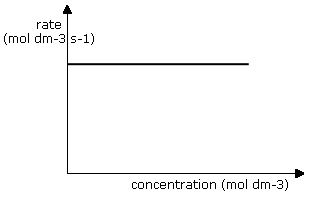
\includegraphics[width=\textwidth]{./Planning/Images/ZeroOrder.jpg}
    \caption{ Rate vs Concentration Zero-Order Graph} \label{fig:Zero Order Graph}
\end{figure}


From the equation you can see that the rate only depends on the rate constant of the reaction. Zero-order reactions occur when the reactant has become exhausted; however before this point is reached, the reaction will follow a different rate law instead of falling to zero directly. There are two general conditions of a reaction that can result in a zero-order reaction:

\begin{itemize}
\item Only a small amount of the reactant molecule are able to react e.g small reacting area/wrong state.
\item When two or more reactants are involved in the reaction the concentrations of some reactants are greater, and therefore overwhelm the other reactants.
\end{itemize}

This usually occurs when a reaction is catalysed by heterogeneous catalysis or to an enzymes specific active site. An example commonly exhibited of this is the decomposition of nitrous oxide.

$N_2O \rightarrow N_2(g) + \dfrac{1}{2} O_2(g)$

The reaction above occurs in the presence of a hot platinum wire catalyst. In this reaction the $N_20$ molecules are limited to the surface area available on the catalyst. Once all of the surface area is occupied at a given time the reaction has an order of zero. This continues until the a part of the surface area is freed up after the products desorb from the catalyst surface and diffuse away$^6$.



\textbf{First-Order Reactions}

A first-order reactions' rate depends linearly on one single reactants concentration. This can be shown by the differential rate equation:

$Rate = k[A]$

The rate constants unit can be obtained mathematically by rearranging the equations units to equal 'k'. When this is done the rate constants unit is s$^{-1}$This equation can also be represented as a rate vs concentration graph. This is shown below and illustrates that the rate of reaction varies only on one single reactants concentration.


\begin{figure}[H]
    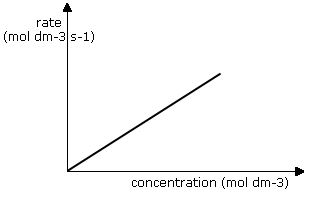
\includegraphics[width=\textwidth]{./Planning/Images/FirstOrder.jpg}
    \caption{ Rate vs Concentration First-Order Graph} \label{fig:First Order Graph}
\end{figure}

\textbf{Second-Order Reactions}

In a second order reaction, the rate equation can be displayed in two ways depending on how the reaction is carried out.

\begin{enumerate}
\item $Rate = k[A] [B]$
\item $Rate = k[A]^2$
\end{enumerate}

Both of these rate equation exhibit a second-order reaction. The first example occurs when the reactants are different and combine in a single step. The first equation shows that if you double A then the rate of reaction is doubled, and the same happens if you double B. For the second example the reactants would have to be identical, and combine in a single step. Therefore doubling A would quadruple the rate of reaction. This means that the rate vs concentration graph would appear to look like the graph below.

\begin{figure}[H]
    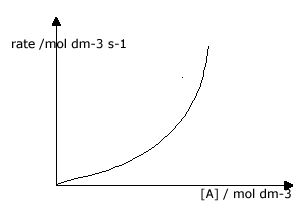
\includegraphics[width=\textwidth]{./Planning/Images/SecondOrder.jpg}
    \caption{ Rate vs Concentration Second-Order Graph} \label{fig:Second Order Graph}
\end{figure}

The rate constants unit can be obtained mathematically by rearranging the equations units to equal 'k'. When this is done the rate constants unit is mol dm$^{-3} s^{-1}$.







	\subsection{Finding Rates}


Rates have to be determined experimentally. The average rate of reaction is obtained by taking the change in concentration over a specific time period. This value is only an approximation of the rate of reaction in that specific time period. This means that this method does not give you the specific rate values throughout that time interval and in some cases, that rate value is not even equal at any time throughout that time interval.

Another method called the instantaneous rate of reaction, in contrast to the average rate of reaction allows for a more accurate value to be obtained. This method is defined as the change in concentration of an infinitely small time interval. The derivative mathematical equation for this is $\frac{d[Concentration]}{dTime}$. By graphing the concentration of the experiment over time you are then able to draw a tangent line at a specific time value. The gradient of the tangent is then directly proportionate to the rate of reaction. You can also mix these two methods to get an average rate which is closer to the value of the instantaneous rate. This is done by measuring the change in concentration over a very small time period, two or more times to obtain an average. Again the rate of reaction for that time period is determined by the slope of the tangent lines$^7$.





		\subsubsection{Justification of Chosen Method}

For my experiment I will be finding the rate of reaction using the following steps:

\begin{enumerate}
\item Plot a graph of the volume of hydrogen against time.
\item From the graph draw a tangent to the line at the initial point.
\item Calculate the gradient of the tangent by using the equation: 
\item The gradient is equal to the rate of reaction.
\end{enumerate}

I have chosen this method as it is the method which will give me the most accurate values for the specific point in time which I wish to measure. 






	\subsection{pH}

The pH scale is composed of two extremes that describes a chemical property about the substance being tested, these extremes are called acids and bases. Mixing acids and bases together will induce a neutralisation reaction which can cancel out their extreme effects. A substance which is neither acidic nor basic is called a neutral substance. The pH scale ranges from 0 to 14, with 0 being as acidic as possible and 14 being as basic as possible. Neutral has a corresponding pH of 7 and therefore anything below 7 is acidic and anything above 7 is basic. The pH scale is illustrated by the following chart.


\begin{figure}[H]
    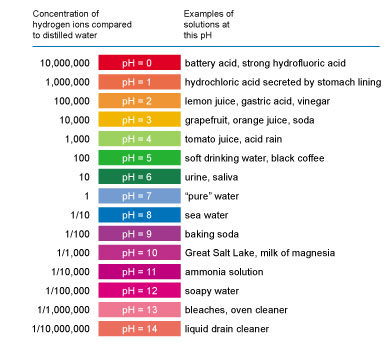
\includegraphics[width=\textwidth]{./Planning/Images/pHScale.jpg}
    \caption{The pH scale} \label{fig:pH Scale}
\end{figure}

The pH scale is a man made scale which is used to measure the concentration of hydrogen ions, each concentration is given a corresponding place on the scale (pH). pH is mathematically defined as the negative logarithm of the hydrogen ion concentration. As a result of this we can determine that the pH scale is logarithmic, therefore each value above/below the neutral value (7) is ten times more basic/acidic respectively. For example pH 6 is ten times as acidic as pH 7  and pH 5 is one hundred times as acidic than pH 7. The mathematical equation for working out pH is illustrated below.

\begin{itemize}
\item $pH = - log [H^+]$
\end{itemize}

There are many indicators used to find out the pH of substances. A table of common indicators with their properties are displayed in the following table.

\begin{figure}[H]
    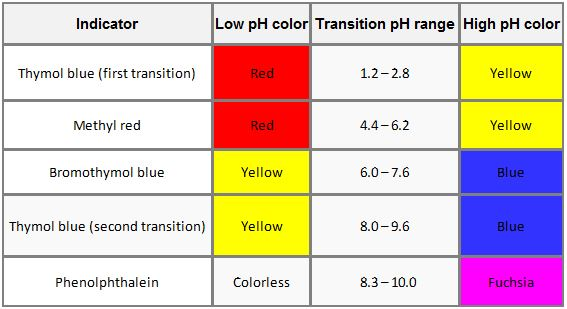
\includegraphics[width=\textwidth]{./Planning/Images/Indicators.jpg}
    \caption{List of pH Indicators} \label{fig:pH Indicators}
\end{figure}

Universal indicator contains all of the chemicals above, all mixed into a single solution or into universal indicator paper. This allows for a continuous colour change from about pH 2 to pH 10. Visual comparison of the colour of the universal indicator and a standard colour chart give a rough reading of the pH of the substance being measured, usually to the nearest whole number. 


	\subsection{Acids}

The Brønsted–Lowry theory defines an acid as a proton H$^+$ donor. They have specific chemical and physical properties. Some of these are detailed in the table below.

\begin{center}
\begin{tabular}{|l|}
    \hline
    \textbf{Acid Properties}  \\ \hline
Piercing pain when placed on a wound. \\ \hline
Tastes sour. \\ \hline
Colourless when placed in phenolphthalein. \\ \hline
Turns blue litmus paper red. \\ \hline
Has a pH value of less than 7. \\ \hline
Produces hydrogen gas when reacted with metals. \\ \hline
Produces carbon dioxide when reacted with carbonates$^8$. \\ \hline
\end{tabular}

\label{tab:Acid Properties}
\end{center}

Acids can be strong or weak depending on their ability to dissociate in water. Strong acids can fully dissociate in water by ionising into H$^+$ ions and the additional anion. These strong acids are usually inorganic acids such as: HCL, HNO$_3$ and H$_2$SO$_4$. Weak acids also dissociate, producing H$^+$ ions and an anion; however these only partially dissociate. This means that in water some molecules will not dissociate as the reaction betwen the ions and the acid is reversible and this equilibrium is in favour of the acid. Weak acids are usually organic acids, such as: Ethanoic acid and benzenol. 

The strength of an acid is not related to its concentration. Both weak and strong acids can be in high concentrations and low concentrations. The concentration refers to the number of moles of the specific acid in a given solution.



	\subsection{Catalysts}

Catalysts are used to speed up the rate of a chemical reaction by finding an alternate pathway of lower activation energy. They do not get used up in a chemical reaction and can be recovered chemically unchanged, often only tiny amounts of catalysts are needed for the catalysts optimum potential$^9$. Although catalysts are not used up in the reaction, they may be destroyed, deactivated or inhibited by a different process. 

A chemical reaction involving a catalyst allows for less energy to be required to reach the transition state, but the total free energy over the process from reactants to products does not change$^{10}$. A catalyst can be involved in multiple steps in a chemical reaction. Catalytic reactions occur in the same way as normal chemical reactions when looking at the kinetics of the reaction (the rate depends on successful collisions of particles). Catalysts do not change the position of the equilibrium. This means, although the initial yield seems to be greater, over time the overall yield would be the same with or without a catalyst. 

Heterogeneous catalysis occurs when the catalyst acts in a different phase to that of the reactants. Generally speaking most heterogeneous catalysts are solids that speed up a reaction involving liquids or gases. A heterogeneous catalyst has active sites which allows a reaction to occur between the reactants. This happens over a 4 step mechanism.

\begin{enumerate}
\item Reactants adsorb onto the catalysts surface.
\item Bonds within the reactants molecules weaken and break.
\item New bonds form to make products.
\item The product desorbs from the catalysts surface and diffuses away.
\end{enumerate}

The active site of the catalyst is only in specific areas due to imperfections in the structure of the catalysts surface at an atomic level. It has been shown that an irregular catalytic surface appears to be more effective than a flat plane surface$^{11}$

Homogeneous catalysis is a chemical reaction that involves a catalyst that is in the same phase of the reactants. Normally homogeneous catalysts are dissolved in a solvent with the reactants. Once the reaction is complete the catalyst is usually released in their initial form, this is why the catalyst is not present in the net reaction equation.

Homogeneous acid catalysis is one of the most common forms of homogeneous catalysis. This is because water is an extremely common solvent which happens to partially dissociate to produce H$^+$ ions. An example of this catalysis is the hydrolysis of esters. As acids catalyse the hydrolysis of esters, carrying out the reaction in water will naturally speed up the reaction, as without any catalytic action the hydrolysis of esters takes a long time. An example acid catalysis is shown below.

$CH_3CO_2CH_3 + H_2O \rightleftharpoons CH_3CO_2H + CH_3OH$




	
	\subsection{Transition Metal Catalysts}

Transition metals are the group of metals in the d block of the periodic table. They are defined as an atom in the d block of the periodic table that has a partially filled d sub-shell and that forms a stable ion. They are divided into three groups:

\begin{itemize}
\item First row transition metals.
\item Second row transition metals.
\item Third row transition metals.
\end{itemize}

Many of these transition metals have catalytic properties, either as a solid metal itself, or a mixed compound. These catalysts work in the same way and are defined in the same way as discussed in the 'Catalyst' section previously.

Transition metals have a number of physical and chemical properties, these are listed in the table below.

\begin{center}
\begin{tabular}{|l|l|}
    \hline
    \textbf{Physical Properties} & \textbf{Chemical Properties} \\ \hline
High melting point & Forms compounds with a variety of oxidation states \\ \hline
High boiling point & Catalytic activity \\ \hline
Good thermal conductivity & Strong tendency to form complexes \\ \hline
Good electrical conductivity & Formation of coloured compounds \\ \hline
High density & \\ \hline
Hard/strong, especially in alloys & \\ \hline
\end{tabular}

\label{tab:Transition Metal Properties}
\end{center}





	\subsection{d Orbitals}

An orbital is defined as a region in an atom where there is a high probability of finding an electron. In total there are 5 different d orbitals. These orbitals are referred to as: $d_z$$^2$, $d_{xy}$, $d_{xz}$, $d_{yz}$ , and $d_x$$^2$$_{-y}$$^2$. These d orbitals are the reason that transition metals have specific physical and chemical properties, as discussed above. As transition metals have a partially filled outermost d sub shell they are able to donate and accept electrons easily, which is why they exhibit catalytic activity. Below shows a representation of the five d orbitals.


\begin{figure}[H]
    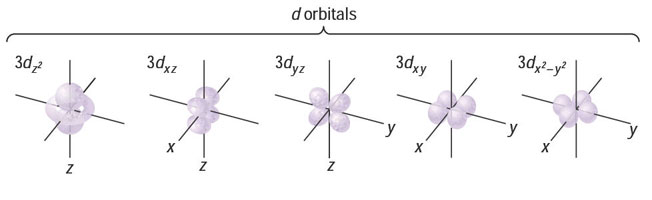
\includegraphics[width=\textwidth]{./Planning/Images/DOrbitals.jpg}
    \caption{d Orbital representations} \label{fig:D Orbitals}
\end{figure}
	

	\subsection{Complexes and their Properties}

A complex is a species that consists of a central metal atom or ion that is surrounded by ligands. Complexes are formed when ligands are bonded to a transition metal by a dative covalent bond. The number of d electrons on the central metal atom or ion is important as transition metals can exist in many different oxidation states which therefore means a different amount of d electrons in the outer shells.  By oxidising or reducing the central metal atom or ion, with the number and type of ligands unchanged, many of the complexes change. These properties include:

\begin{itemize}
\item Reactivity.
\item Magnetic Activity.
\item Stability.
\item Stereochemistry.
\item Spectroscopic properties.
\end{itemize}

Complexes contain a coordination number which identifies the number of dative bonds that are formed from the surrounding ligands to the central metal atom or ion. Usually the coordination number is: 2, 4 or 6. Each coordination number causes a different shaped complex. These different shapes are outlined below.

\begin{figure}[H]
    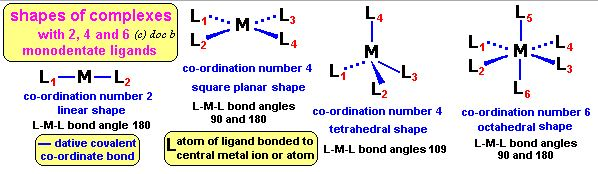
\includegraphics[width=\textwidth]{./Planning/Images/ComplexShapes.jpg}
    \caption{Complex Shapes and Structures} \label{fig:Complex Shapes}
\end{figure}




	\subsection{Enthalpy Level Diagrams}	

Enthalpy is the heat energy content of a substance. The net heat energy transferred to a system from the surroundings to a system at constant pressure is known as the enthalpy change ($\Delta H$). This can be worked out mathematically by applying the formula:

$\Delta H^\circ = \sum {H^\circ _f {\rm{products}}} - \sum {H^\circ _f {\rm{reactants}}}$

An exothermic reaction would produce a negative $\Delta H$ value as the enthalpy of the reaction system is decreasing. This occurs as heat energy is given out from the system to the surroundings. 

\begin{figure}[H]
    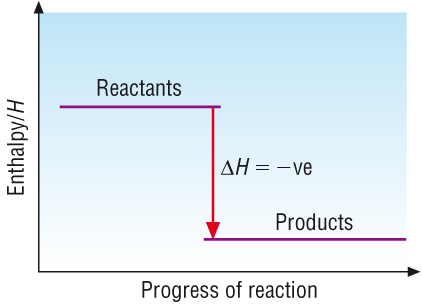
\includegraphics[width=\textwidth]{./Planning/Images/Exothermic.jpg}
    \caption{Exothermic Enthalpy Diagram} \label{fig:Exothermic}
\end{figure}

An endothermic reaction would produce a positive $\Delta H$ value as the enthalpy of the reaction system is increasing. This occurs as heat energy is absorbed in from the surroundings.

\begin{figure}[H]
    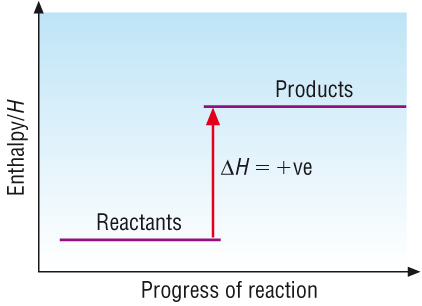
\includegraphics[width=\textwidth]{./Planning/Images/Endothermic.jpg}
    \caption{Endothermic Enthalpy Diagram} \label{fig:Endothermic}
\end{figure}


All enthalpy equations are carried out under standard conditions which has 3 criteria.

\begin{enumerate}
\item 298K.
\item 1ATM.
\item 1 Molar Solutions.
\end{enumerate}

The state symbols also need to be involved as the molecules have different amounts of energy in different states.



\section{Inventory}

	\subsection{Equipment List}
\begin{itemize}
\item 250 $cm^3$ conical flask.
\item Bung fitted to a glass tube.
\item Burette.
\end{itemize}

	\subsection{Chemical List}
\begin{itemize}
\item Distilled Water.
\item 0.20 mol dm$^-3$ Copper Sulfate ${_(aq)}$.
\item 1.0 mol dm$^-3$ Sulfuric Acid${_(aq)}$.
\item Granulated Zinc${_(s)}$.
\item Mixture of Different Catalysts.
\end{itemize}



\section{Methods}

	\subsection{Chosen Method}

\textbf{Setting Up}

\begin{enumerate}
\item Fill the burette with distilled water.
\item Fit the bung (fitted with glass tube) into the conical flask.
\item Fit the inverted burette to the end of the glass tube.
\end{enumerate}

\textbf{Carrying out the Experiment}

\begin{enumerate}
\item Remove the bung from the conical flask and pour 30 cm$^3$ of distilled water and 10 cm$^3$ of sulfuric acid into the conical flask.
\item Weigh out 1.0 g of granulated zinc.
\item Add the measured 1.0 g of granulated zinc to the conical flask.
\item Place the bung back in the conical flask.
\item Record the volume of hydrogen produced in cm$^3$ every 30 seconds for 5 minutes from the burette markings to 1 decimal place.
\item Repeat the experiment but use 30 cm$^3$ of copper sulfate instead of distilled water.
\end{enumerate} 

\textbf{Interpreting the Data (as discussed before)}

\begin{enumerate}
\item Plot a graph of the volume of hydrogen against time.
\item From the graph draw a tangent to the line at the initial point.
\item Calculate the gradient of the tangent by using the equation: 
\item The gradient is equal to the rate of reaction.
\end{enumerate}



	\subsection{Justification of Chosen Method}

In addition to the method discussed above, there are two other methods which would allow me to carry out my experiment:
\begin{itemize}
\item The Gas Syringe Method
\item The Mass Change Method 
\end{itemize}

Below, the methods are explained:

\textbf{Gas Syringe Method}



Setting up involves a similar set up to my chosen method, but the gas syringe replaces the burette. This is shown below:
\begin{figure}[H]
    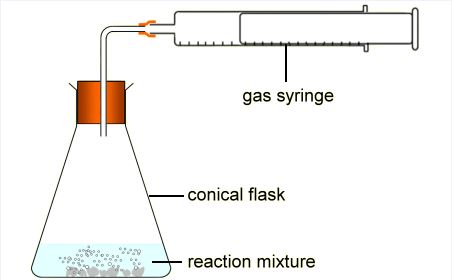
\includegraphics[width=\textwidth]{./Planning/Images/GasSyringe.jpg}
    \caption{Gas Syringe Equipment} \label{fig:Gas Syringe}
\end{figure}

Carrying out the method is precisely the same as my chosen method except a reading is taken from the gas syringe instead of the burette. This is precisely the reason I have chosen to not use this method. The gas syringes available to me have graduations every 1 ml, whereas the burettes available to me have graduations every 0.1 ml. Therefore the accuracy of my readings will be greater using the burette method and consequently I have chosen the burette method over the gas syringe method. 

\textbf{Mass Change Method}

Setting up this method involves:
\begin{itemize}
\item Balance (reading to 0.01 g)
\item Conical Flask
\item Cotton Wool
\end{itemize}

\begin{figure}[H]
    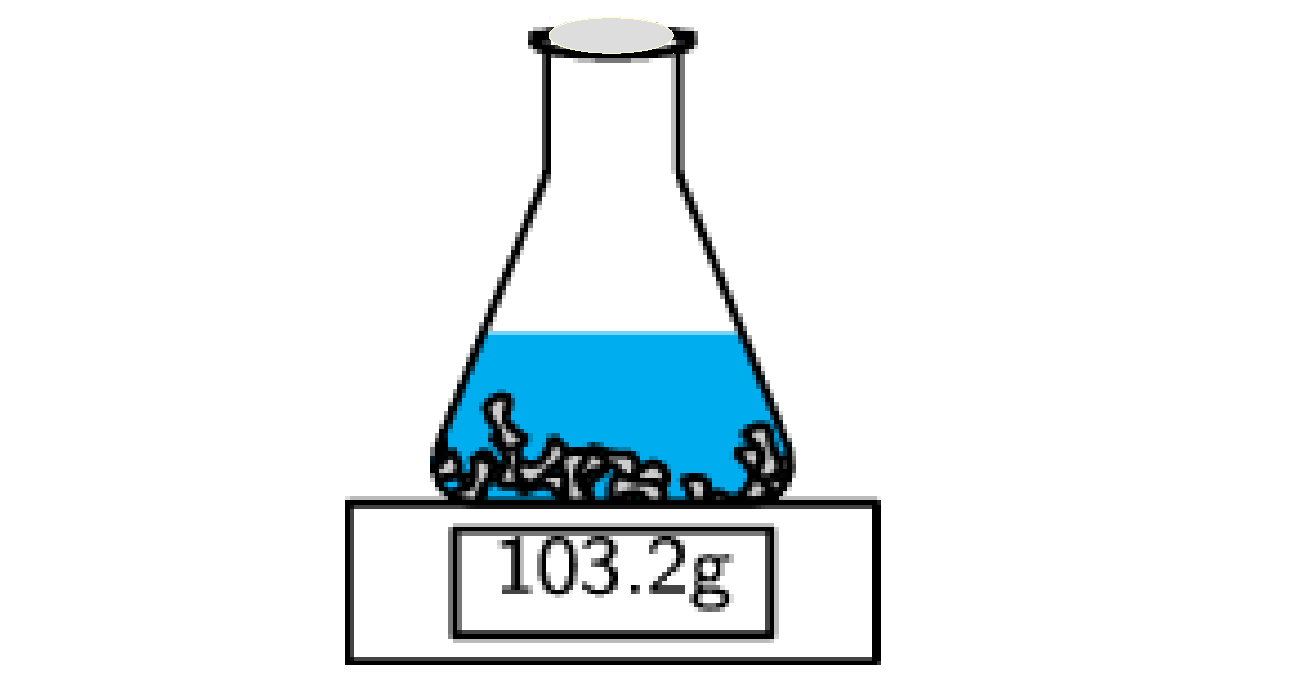
\includegraphics[width=\textwidth]{./Planning/Images/MassChange.pdf}
    \caption{Mass Change Experiment} \label{fig:Mass Change}
\end{figure}


Carrying out this method involves:

\begin{enumerate}
\item Zero the Balance.
\item Pour 30 cm$^3$ of distilled water and 10 cm$^3$ of sulfuric acid into the conical flask.
\item Take note of the Balance value + 1.0 g
\item Weigh out 1.0 g of granulated zinc.
\item Add the measured 1.0 g of granulated zinc to the conical flask.
\item Place the cotton wool in the conical flask to stop acid 'spray' escaping.
\item Record the loss in mass in grams every 30 seconds for 5 minutes to 2 decimal places.
\item Repeat the experiment but use 30 cm$^3$ of copper sulfate instead of distilled water.
\end{enumerate} 

I have chosen not to carry out this method as the balance will be a lot more sensitive to the environment and there will be room for a lot more human error. For example, left over residue could land on the scales and skew the results during the experiment. 


\begin{landscape}

\section{Risk Assessment}

\begin{center}
\begin{longtable}{|p{1.5cm}|p{1.5cm}|p{3cm}|p{3cm}|p{3cm}|p{3cm}|p{2cm}|}
    \hline
 \textbf{Name of Chemical} & \textbf{Source of Information} & \textbf{Hazards} & \textbf{Risks} & \textbf{Control Measures} & \textbf{Disposal Method} & \textbf{Emergency Procedures} \\ \hline

Copper Sulfate (aq) &
CLEAPSS Hazcards &
\begin{itemize}
\item Harmful
\item Dangerous for the Environment \end{itemize} &
\begin{itemize}
\item Harmful if swallowed
\item Irritating to eyes and skin \end{itemize} &
\begin{itemize}
\item Do not put near mouth
\item Use gloves
\item Use goggles
\item Keep away from water, unless intended. \end{itemize} & 
Dissolve 64 g in 1 litre of water before pouring the solution down a foulwater drain. This disposal procedure should be kept to a minimum. &
Seek medical attention. Wash contaminated area. \\ \hline

Hydrated Copper Sulfate (s) &
CLEAPSS Hazcards &
\begin{itemize}
\item Harmful
\item Dangerous for the Environment \end{itemize} &
\begin{itemize}
\item Harmful if swallowed
\item Irritating to eyes and skin \end{itemize} &
\begin{itemize}
\item Do not put near mouth
\item Use gloves
\item Use goggles
\item Label: Harmful, if above 1 mol dm$^-3$ \end{itemize} &
Crystals may be used for solutions. Dilute to less than 0.4 mol dm$^-3$ or dissolve 100 g in 1 litre of water before pouring the solution down a foul-water drain. This disposal procedure should be kept to a minimum . &
Seek medical attention. Wash contaminated area. \\ \hline



Sulfuric Acid (aq) &
CLEAPSS Hazcards &
\begin{itemize}
\item Corrosive
\item Irritant \end{itemize} &
Causes serious burns & 
\begin{itemize}
\item Label: Irritant, if above 0.5 mol dm$^-3$
\item Label: Corrosive, if above 1.5 mol dm$^-3$
\item Wear gloves
\item Wear goggles \end{itemize} &
Add slowly no more than 10 cm$^3$ of concentrated sulfuric(VI) acid to 1 litre of 1 mol dm$^-3$ sodium carbonate solution (containing indicator) which should be constantly stirred. Let the mixture cool (or add ice), before adding more acid. Pour the solution down a foul-water drain. & 
Remove contaminated clothing and quickly wipe as much liquid as possible off the skin with a dry cloth before drenching the area with a large excess of water. If a large area is affected or blistering occurs, seek medical attention. \\ \hline

Granulated Zinc (s) &
CLEAPSS Hazcards &
\begin{itemize}
\item Low Hazard \end{itemize} &
N/A &
Place in normal refuse &
N/A &
N/A \\ \hline

\end{longtable}
\label{tab:Risk Assessment Table}

\end{center}


\end{landscape}



